\documentclass{article}
\usepackage{amsmath}

\usepackage{graphicx}
\usepackage{hyperref}
\usepackage{float}
\usepackage{csvsimple}

\graphicspath{./images/}

\title{Rapport de laboratoire: \\Intelligence Artificielle}
\author{Matthias Léonard et Dawid Krasowski}
\date{2022/2023}

\begin{document}
\maketitle

\begin{figure}[h]
    \centering
    
\includegraphics[scale=0.15]{./images/Logo ECAM.png}

\end{figure}


\paragraph{Superviseur :} Monsieur HASSELMANN Ken



\pagebreak
\tableofcontents
\pagebreak
\section{Introduction}

    Dans le cadre des laboratoires d'intelligence artificielle dispensé à l'ECAM en 2ème Master en ingénieur informatique.
Sous la supervision de Monsieur HASSELMANN notre projet se base sur la recherche de fraude à la carte bancaire.
Nous travaillons sur un jeu de données de transactions bancaires issues d'Ouganda 
ces données on été fournis lors d'une compétition Xente de 2019.\\ \url{https://zindi.africa/competitions/xente-fraud-detection-challenge} \\

Notre projet est disponible sur GitHub à l'adresse suivante :\\ \url{https://github.com/LeTouristeDeLECAM/Lab_AI_Fraud_Detection} \\
Pour des questions de propriété et droit les données ne sont pas disponibles sur GitHub.


\section{Présentation des données}
\subsection{Description des données}

% Added description table 
\begin{table}[h]
\centering
\csvautotabular{../../Data/Xente_Variable_Definitions.csv}
\caption{Description des données}
\end{table}

\subsection{identification des Features}
Dans un premier temps nous cherchons à identifier les features qui vont nous permettre de créer un modèle de prédiction de fraude.\\

Nous pouvons observer que certaines données ne sont pas utile pour obtenir un modèle. 
Nous décidons de supprimer les colonnes suivantes :
\begin{itemize}
    \item CurrencyCode : Toutes les transactions sont en UGX soit en Shilling Ougandais.
    \item CountryCode : Toutes les transactions sont en Ouganda.
\end{itemize} 
Nous pouvons également imaginer à première vue que les données Amount et Value sont similaires.
Néanmoins suite à une analyse: \\ \\
%Italique
\emph{diff = test2["Amount"] - abs(test2["Value"])\\diff.describe()}\\

nous pouvons observer que les deux colonnes ne sont pas totalement identiques.\\
% ajout de la table csv
\begin{table}[h]
    \centering
    \csvautotabular{./images/Amout_Value_description.csv}
    \caption{Description statistique de la différence entre Amount et Value}
        
 \end{table}

Nous avons décidé de garder les données Amount et Value. Car sur les 193 fraudes que comporte le jeu de données, 
17  fraudes sont réalisé quand Amount et Value sont différents (8,8\%).\\

\paragraph{Features à supprimer :}
% figure import 
\begin{figure}[h]
    \centering
    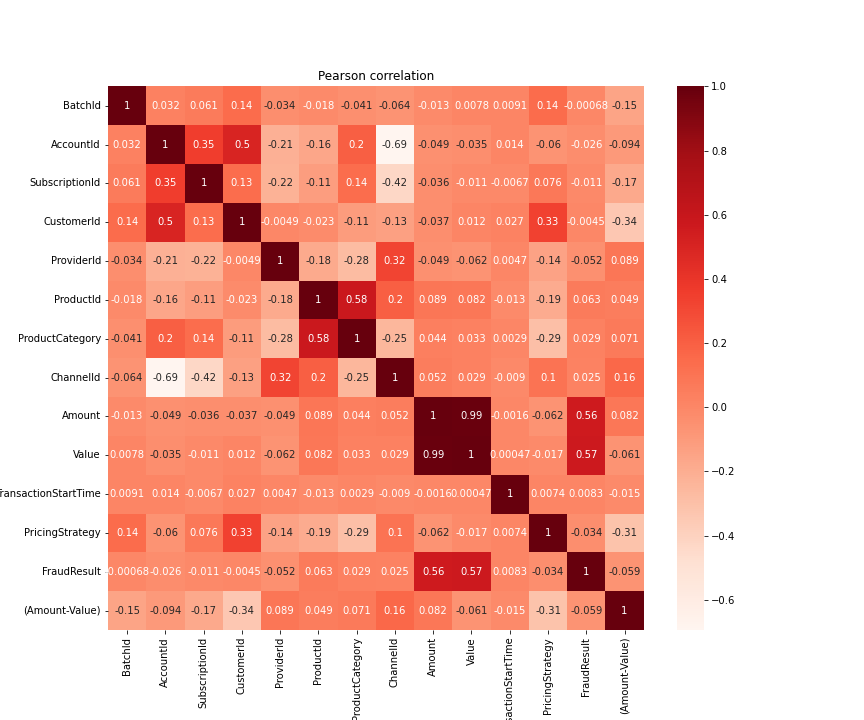
\includegraphics[scale=0.4]{./images/correlation_pearson.png}
    \caption{Corrélation de Pearson entre les features} 
\end{figure}





Nous pouvons observer que productCategory et productID sont fortement corrélés.
il en est de même pour amount et value.\\

Pour pousuivre notre analyse nous réalisons une analyse en composante principale (ACP) sur les données.\\
Cette analyse nous permet de réduire la dimensionnalité de nos données et identifier les données qui sont les plus importantes.\\

\section{Conclusion}
Nous avons observé une diminution de la divergence.
\end{document}
